% Options for packages loaded elsewhere
\PassOptionsToPackage{unicode}{hyperref}
\PassOptionsToPackage{hyphens}{url}
\PassOptionsToPackage{dvipsnames,svgnames,x11names}{xcolor}
%
\documentclass[
  letterpaper,
  DIV=11,
  numbers=noendperiod]{scrartcl}

\usepackage{amsmath,amssymb}
\usepackage{lmodern}
\usepackage{iftex}
\ifPDFTeX
  \usepackage[T1]{fontenc}
  \usepackage[utf8]{inputenc}
  \usepackage{textcomp} % provide euro and other symbols
\else % if luatex or xetex
  \usepackage{unicode-math}
  \defaultfontfeatures{Scale=MatchLowercase}
  \defaultfontfeatures[\rmfamily]{Ligatures=TeX,Scale=1}
\fi
% Use upquote if available, for straight quotes in verbatim environments
\IfFileExists{upquote.sty}{\usepackage{upquote}}{}
\IfFileExists{microtype.sty}{% use microtype if available
  \usepackage[]{microtype}
  \UseMicrotypeSet[protrusion]{basicmath} % disable protrusion for tt fonts
}{}
\makeatletter
\@ifundefined{KOMAClassName}{% if non-KOMA class
  \IfFileExists{parskip.sty}{%
    \usepackage{parskip}
  }{% else
    \setlength{\parindent}{0pt}
    \setlength{\parskip}{6pt plus 2pt minus 1pt}}
}{% if KOMA class
  \KOMAoptions{parskip=half}}
\makeatother
\usepackage{xcolor}
\usepackage[bottom=30mm,top=25mm,left=22mm,right=22mm]{geometry}
\setlength{\emergencystretch}{3em} % prevent overfull lines
\setcounter{secnumdepth}{-\maxdimen} % remove section numbering
% Make \paragraph and \subparagraph free-standing
\ifx\paragraph\undefined\else
  \let\oldparagraph\paragraph
  \renewcommand{\paragraph}[1]{\oldparagraph{#1}\mbox{}}
\fi
\ifx\subparagraph\undefined\else
  \let\oldsubparagraph\subparagraph
  \renewcommand{\subparagraph}[1]{\oldsubparagraph{#1}\mbox{}}
\fi


\providecommand{\tightlist}{%
  \setlength{\itemsep}{0pt}\setlength{\parskip}{0pt}}\usepackage{longtable,booktabs,array}
\usepackage{calc} % for calculating minipage widths
% Correct order of tables after \paragraph or \subparagraph
\usepackage{etoolbox}
\makeatletter
\patchcmd\longtable{\par}{\if@noskipsec\mbox{}\fi\par}{}{}
\makeatother
% Allow footnotes in longtable head/foot
\IfFileExists{footnotehyper.sty}{\usepackage{footnotehyper}}{\usepackage{footnote}}
\makesavenoteenv{longtable}
\usepackage{graphicx}
\makeatletter
\def\maxwidth{\ifdim\Gin@nat@width>\linewidth\linewidth\else\Gin@nat@width\fi}
\def\maxheight{\ifdim\Gin@nat@height>\textheight\textheight\else\Gin@nat@height\fi}
\makeatother
% Scale images if necessary, so that they will not overflow the page
% margins by default, and it is still possible to overwrite the defaults
% using explicit options in \includegraphics[width, height, ...]{}
\setkeys{Gin}{width=\maxwidth,height=\maxheight,keepaspectratio}
% Set default figure placement to htbp
\makeatletter
\def\fps@figure{htbp}
\makeatother

\usepackage{booktabs}
\usepackage{longtable}
\usepackage{array}
\usepackage{multirow}
\usepackage{wrapfig}
\usepackage{float}
\usepackage{colortbl}
\usepackage{pdflscape}
\usepackage{tabu}
\usepackage{threeparttable}
\usepackage{threeparttablex}
\usepackage[normalem]{ulem}
\usepackage{makecell}
\usepackage{xcolor}
\KOMAoption{captions}{tableheading}
\usepackage{titling}
\usepackage{hyperref}
\usepackage{multirow}
\pretitle{\begin{center}\fontsize{18bp}{18bp}\selectfont}
\posttitle{\par\end{center}}
\usepackage[font=small]{caption} \captionsetup[table]{labelformat=empty} \captionsetup[figure]{labelformat=empty}
\preauthor{\begin{center}\fontsize{11bp}{11bp}\selectfont}
\postauthor{\par\end{center}\vspace{24bp}}
\predate{}
\date{}
\postdate{}
\usepackage[most]{tcolorbox}
\usepackage{ragged2e}
\definecolor{yellow}{rgb}{0.98, 0.88, 0.71}
\newtcolorbox{myquote}{colback=yellow, grow to right by=1mm, grow to left by=-1mm, boxrule=0pt,boxsep=0pt,breakable}
\newcommand{\todo}[1]{\begin{myquote}  \normalsize{#1} \end{myquote}}
\makeatletter
\makeatother
\makeatletter
\makeatother
\makeatletter
\@ifpackageloaded{caption}{}{\usepackage{caption}}
\AtBeginDocument{%
\ifdefined\contentsname
  \renewcommand*\contentsname{Table of contents}
\else
  \newcommand\contentsname{Table of contents}
\fi
\ifdefined\listfigurename
  \renewcommand*\listfigurename{List of Figures}
\else
  \newcommand\listfigurename{List of Figures}
\fi
\ifdefined\listtablename
  \renewcommand*\listtablename{List of Tables}
\else
  \newcommand\listtablename{List of Tables}
\fi
\ifdefined\figurename
  \renewcommand*\figurename{Figure}
\else
  \newcommand\figurename{Figure}
\fi
\ifdefined\tablename
  \renewcommand*\tablename{Table}
\else
  \newcommand\tablename{Table}
\fi
}
\@ifpackageloaded{float}{}{\usepackage{float}}
\floatstyle{ruled}
\@ifundefined{c@chapter}{\newfloat{codelisting}{h}{lop}}{\newfloat{codelisting}{h}{lop}[chapter]}
\floatname{codelisting}{Listing}
\newcommand*\listoflistings{\listof{codelisting}{List of Listings}}
\makeatother
\makeatletter
\@ifpackageloaded{caption}{}{\usepackage{caption}}
\@ifpackageloaded{subcaption}{}{\usepackage{subcaption}}
\makeatother
\makeatletter
\@ifpackageloaded{tcolorbox}{}{\usepackage[many]{tcolorbox}}
\makeatother
\makeatletter
\@ifundefined{shadecolor}{\definecolor{shadecolor}{rgb}{.97, .97, .97}}
\makeatother
\makeatletter
\makeatother
\ifLuaTeX
  \usepackage{selnolig}  % disable illegal ligatures
\fi
\IfFileExists{bookmark.sty}{\usepackage{bookmark}}{\usepackage{hyperref}}
\IfFileExists{xurl.sty}{\usepackage{xurl}}{} % add URL line breaks if available
\urlstyle{same} % disable monospaced font for URLs
\hypersetup{
  colorlinks=true,
  linkcolor={black},
  filecolor={Maroon},
  citecolor={Blue},
  urlcolor={blue},
  pdfcreator={LaTeX via pandoc}}

\title{\LARGE Microbial diversity decline and community response are
decoupled from increased respiration in warmed tropical forest soil\\
\strut \\
Extended Data}
\author{Andrew T. Nottingham\textsuperscript{1,2,3*}, Jarrod J.
Scott\textsuperscript{3}, Kristin Saltonstall\textsuperscript{3}, Kirk
Broders\textsuperscript{3,4},\\
Maria Montero-Sanchez\textsuperscript{3}, Johann
Püspök\textsuperscript{3}, Erland Bååth\textsuperscript{5}, Patrick
Meir\textsuperscript{2,6}\\
\strut \\
\strut \\
\RaggedRight \small \textsuperscript{1}School of Geography, University
of Leeds, Leeds, UK\\
\small \textsuperscript{2}School of Geosciences, University of
Edinburgh, Crew Building, Kings Buildings, Edinburgh, UK\\
\small \textsuperscript{3}Smithsonian Tropical Research Institute,
0843-03092, Balboa, Ancon, Republic of Panama\\
\small \textsuperscript{4}USDA, Agricultural Research Service, National
Center for Agricultural Utilization Research, Peoria, IL, USA\\
\small \textsuperscript{5}Section of Microbial Ecology, Department of
Biology, Lund University, 22362, Lund, Sweden.\\
\small \textsuperscript{6}Research School of Biology, Australian
National University, Canberra, ACT 2601, Australia\\
\strut \\
\small \textsuperscript{*}Corresponding author:
A.Nottingham@leeds.ac.uk}
\date{}

\begin{document}
\maketitle
\ifdefined\Shaded\renewenvironment{Shaded}{\begin{tcolorbox}[borderline west={3pt}{0pt}{shadecolor}, interior hidden, breakable, sharp corners, enhanced, boxrule=0pt, frame hidden]}{\end{tcolorbox}}\fi

\begin{figure}

{\centering 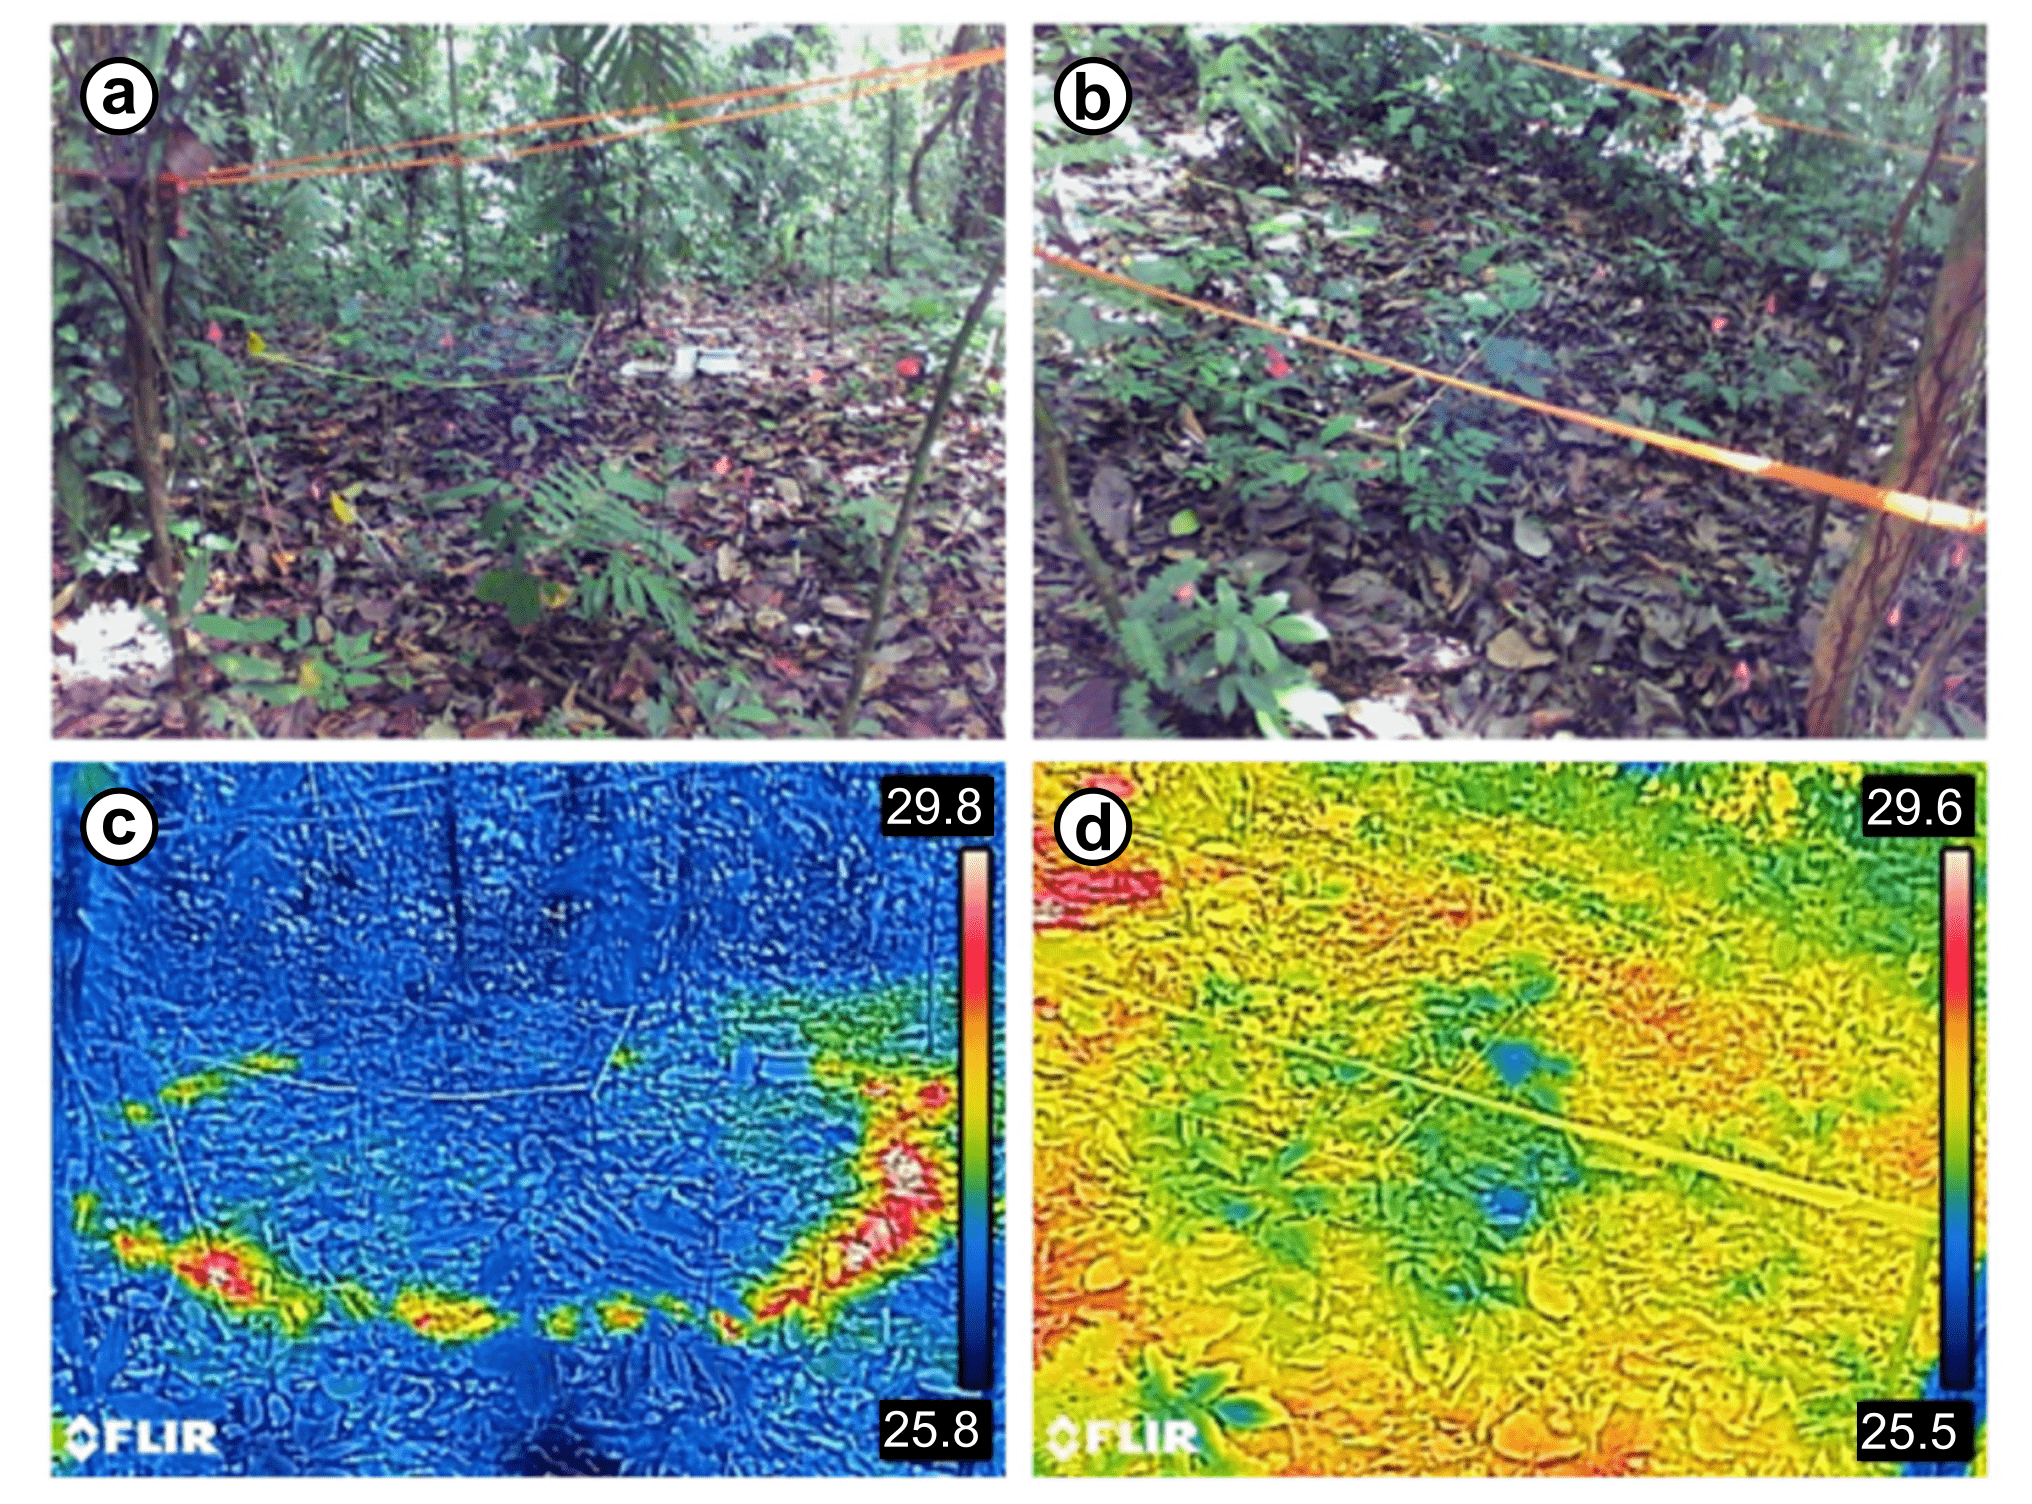
\includegraphics[width=1\textwidth,height=\textheight]{FIGURES/Extended_Data_Fig_1.png}

}

\caption{\textbf{Extended Data Figure 1 |}
\textbf{One of five warmed plots at SWELTR.} The images show the soil
surface temperature shortly after the warming structure was switched on
(\textbf{a} and \textbf{c}) and after a period of thermal equilibration`
(\textbf{b} and \textbf{d}). The circular heating structure was 3.5 m in
diameter and extended to 1.2 m depth, which resulted in an effective
heated plot of approximately 5 m diameter x \textgreater{} 1.5 m depth
(i.e.~to the bedrock, situated at around 1.5--2.0 m across the study
site). The experiment consisted of five warmed and control plot-pairs in
total.}

\end{figure}

\begin{figure}

{\centering \includegraphics[width=0.73\textwidth,height=\textheight]{FIGURES/Extended_Data_Fig_2.png}

}

\caption{\textbf{Extended Data Figure 2 |}
\textbf{Diversity response of soil bacteria (a--c) and fungi (d--f) to two years of warming by +3°C and +8°C}.
Shapiro-Wilk Normality and Bartlett tests indicated all alpha diversity
estimates (following PERfect filtering) wer normally distributed and
differences were assessed for (\textbf{a}) bacteria and (\textbf{d})
fungi using analysis of variance (ANOVA) followed by Tukey HSD post hoc
tests. Compositional similarity of microbial communities
(beta-diversity) represented as PCoA ordination plots of PERfect
filtered data for (\textbf{b}) bacteria---estimated using Unweighted
(left) and Weighted Unifrac (right) distance matrices; and (\textbf{e})
fungi estimated---using Jensen--Shannon divergence (left) and
Bray-Curtis (right) distance matrices. Within group distances for the
(\textbf{c}) bacteria and (\textbf{f}) fungi datasets. The centre line
of each box plot represents the median, the lower and upper hinges
represent the first and third quartiles and whiskers represent + 1.5 the
interquartile range. Significant differences denoted by asterisks (* p
\(\le\) 0.05, ** p \(\le\) 0.01, *** p \(\le\) 0.001, **** p \(\le\)
0.0001).}

\end{figure}

\begin{figure}

{\centering \includegraphics[width=1\textwidth,height=\textheight]{FIGURES/Extended_Data_Fig_3.png}

}

\caption{\textbf{Extended Data Figure 3 |}
\textbf{The response of select soil bacteria taxa to two years of warming by +3°C and +8°C}.
Differences assessed for multiple-group pair-wise comparisons using
ANOVA followed by Tukey HSD post hoc tests. PERfect filtered read count
data was log\(_{10}\) transformed and normalized using total sum scaling
(TSS). The centre line of each box plot represents the median, the lower
and upper hinges represent the first and third quartiles and whiskers
represent + 1.5 the interquartile range. Significant differences denoted
by asterisks (* p \(\le\) 0.05, ** p \(\le\) 0.01, *** p \(\le\) 0.001,
**** p \(\le\) 0.0001).}

\end{figure}

\begin{figure}

{\centering \includegraphics[width=1\textwidth,height=\textheight]{FIGURES/Extended_Data_Fig_4.png}

}

\caption{\textbf{Extended Data Figure 4 |}
\textbf{The response of select soil fungal taxa to two years of warming by +3°C and +8°C}.
Differences assessed for multiple-group pair-wise comparisons using
ANOVA followed by Tukey HSD post hoc tests. PERfect filtered read count
data was log\(_{10}\) transformed and normalized using total sum scaling
(TSS). The centre line of each box plot represents the median, the lower
and upper hinges represent the first and third quartiles and whiskers
represent + 1.5 the interquartile range. Significant differences denoted
by asterisks (* p \(\le\) 0.05, ** p \(\le\) 0.01, *** p \(\le\) 0.001,
**** p \(\le\) 0.0001).}

\end{figure}

\begin{figure}

{\centering \includegraphics[width=0.85\textwidth,height=\textheight]{FIGURES/Extended_Data_Fig_5.png}

}

\caption{\textbf{Extended Data Figure 5 |}
\textbf{Distance-based Redundancy Analysis (db-RDA)} of PIME filtered
data based on Bray-Curtis dissimilarity showing the relationships
between community composition change for (\textbf{a}) bacteria and
(\textbf{b}) fungi versus edaphic properties (left) and microbial
functional response (right).}

\end{figure}

\begin{figure}

{\centering 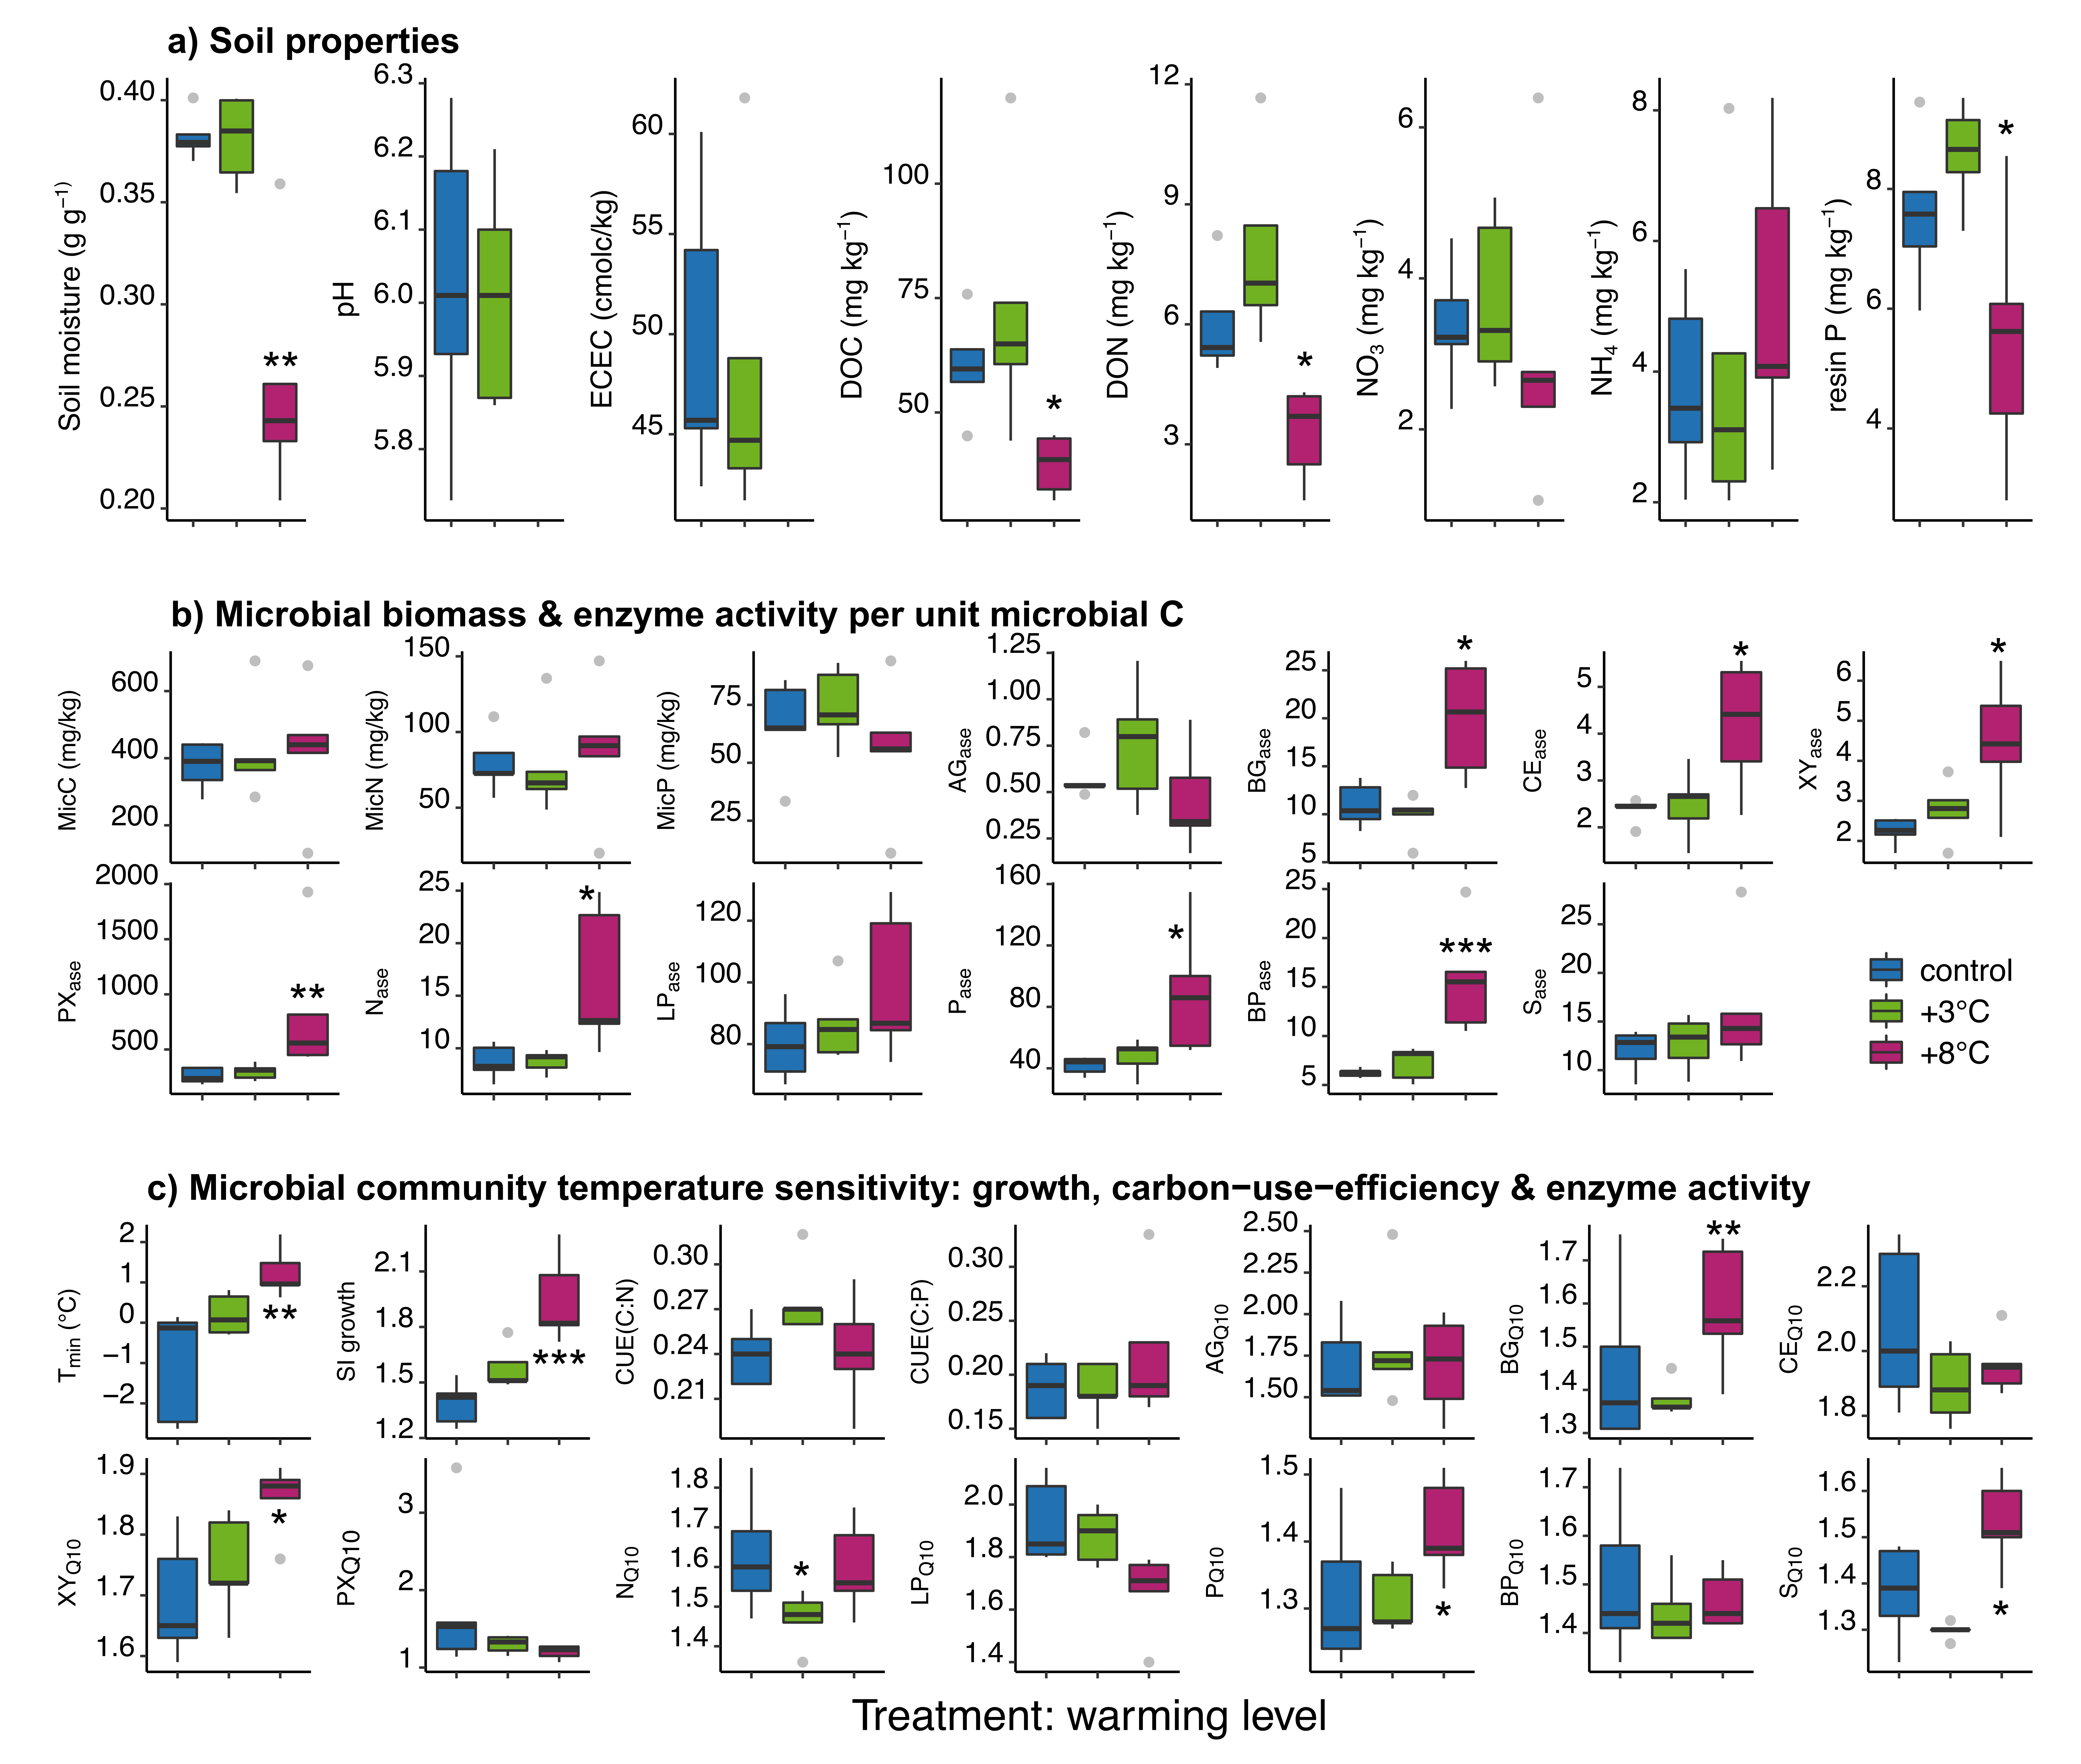
\includegraphics[width=1\textwidth,height=\textheight]{FIGURES/Extended_Data_Fig_6.png}

}

\caption{\textbf{Extended Data Figure 6 |}
\textbf{Soil, enzyme, and microbial responses to +3ºC and +8ºC \textsl{in situ} soil warming.}
Data are grouped by (\textbf{a}) soil properties, (\textbf{b}) microbial
functional responses, and (\textbf{c}) microbial temperature adaptive
responses; we used the same grouping to test three hypotheses on how
each of these responses were correlated to changes in microbial
diversity and community composition (Fig. 2; Extended data: Table 2,
Fig. 5). All properties were determined for soil samples collected
during the 2018 wet season (June and November); see methods. Units for
enzyme V\(_{\mathrm{max}}\) are nmol MU g\(^{-1}\) min\(^{-1}\), except
Phenol oxidase in \(\mu\)mol g\(^{-1}\) h\(^{-1}\) and Leucine
aminopeptidase in nmol AMC g\(^{-1}\) min\(^{-1}\). The centre line of
each box plot represents the median, the lower and upper hinges
represent the first and third quartiles and whiskers represent + 1.5 the
interquartile range. Significant differences between treatments and
controls are highlighted by asterisks (ANOVA; * p \(\le\) 0.05, ** p
\(\le\) 0.01, *** p \(\le\) 0.001). For n = 5 plots.}

\end{figure}

\begin{figure}

{\centering 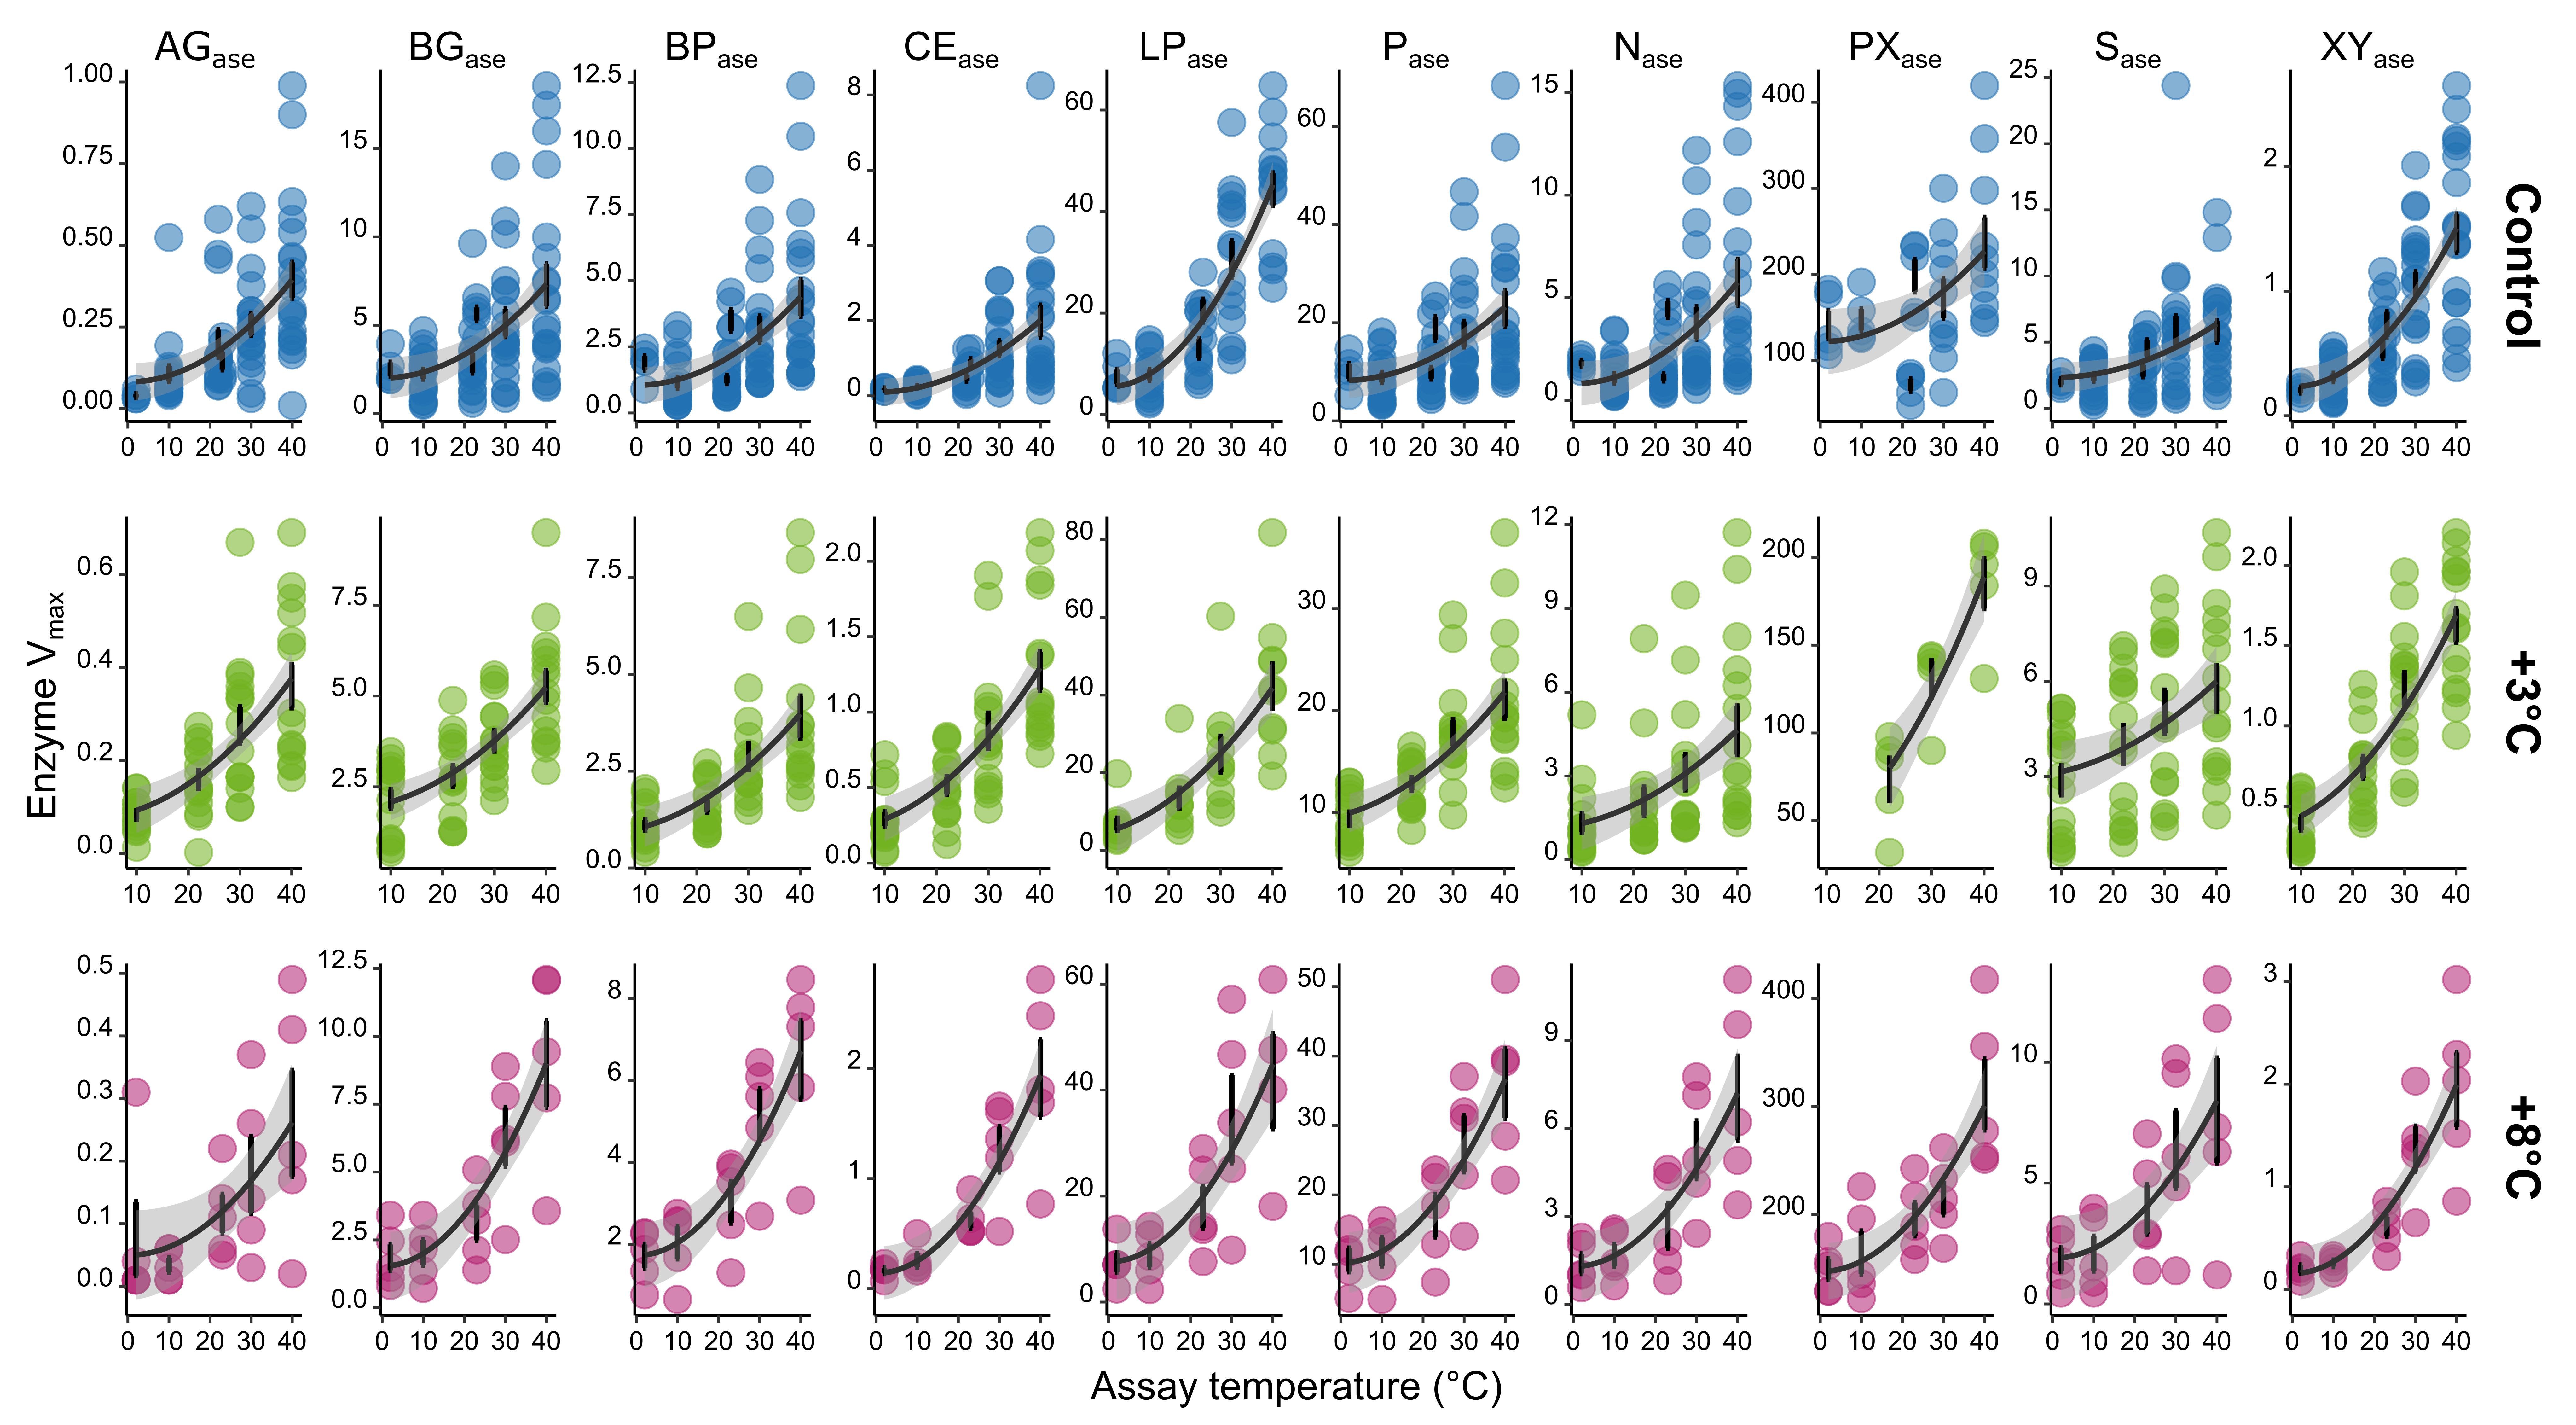
\includegraphics[width=1\textwidth,height=\textheight]{FIGURES/Extended_Data_Fig_7.png}

}

\caption{\textbf{Extended Data Figure 7 |}
\textbf{Soil enzyme activities in response to incubation temperature (i.e. instantaneous temperature response determined in laboratory assays).}
Data are maximum potential enzyme activity (V\(_{\mathrm{max}}\)),
determined by activity under saturating substrate conditions. Enzymes
are: \(\alpha\)-glucosidase (AG\(_{\mathrm{ase}}\)),
\(\beta\)-glucosidase (BG\(_{\mathrm{ase}}\)), phospho-diesterase
(BP\(_{\mathrm{ase}}\)), cellolbiohydrolase (CE\(_{\mathrm{ase}}\)),
leucine aminopeptidase (LP\(_{\mathrm{ase}}\)), phosphomonoesterase
(P\(_{\mathrm{ase}}\)), \textsl{N}-acetyl \(\beta\)-glucosaminidase
(N\(_{\mathrm{ase}}\)), phenol oxidase (PX\(_{\mathrm{ase}}\)),
sulfatase (S\(_{\mathrm{ase}}\)) and \(\beta\)-xylanase
(XY\(_{\mathrm{ase}}\)). Units for enzyme V\(_{\mathrm{max}}\) are nmol
MU g\(^{-1}\) min\(^{-1}\), except Phenol oxidase in \(\mu\)mol
g\(^{-1}\) h\(^{-1}\) and Leucine aminopeptidase in nmol AMC g\(^{-1}\)
min\(^{-1}\). All data are for are for n = 10 plots, determined during
the wet season 2018. Controls include 4 sampling periods (June, Sept,
Oct, Dec 2018); +3°C include 3 sampling periods (June, Sept, Dec 2018);
+8°C include 1 sampling period (Sept 2018).}

\end{figure}

\begin{table}[H]

\caption{\textbf{Extended Data Table 1 |} \textbf{Relationship of bacterial and fungal richness with (a) environmental drivers, (b) microbial functional responses and (c) microbial temperature adaptive responses}. For environmental drivers of richness (\textbf{a}), we included temperature, moisture and key edaphic properties: models included fixed effects of Environmental drivers: treatment level (warming by +3°C and +8°C), soil moisture, soil properties (pH, N, resin P and ECEC), treatment:moisture interaction. For microbial functional correlates of richness (\textbf{b}), we included CO$_{2}$ efflux, microbial C and activity of four enzymes (V$_{\mathrm{max}}$ for phosphomonoesterase, $\beta$-glucosidase, $\beta$-xylanase and \textsl{N}-acetyl $\beta$-glucosaminidase). For microbial temperature adaptation correlates of richness (\textbf{c}), we included CUE (determined by C:N and C:P ratios of enzymatic activity), the temperature sensitivity (\textsl{Q}$_{10}$) of four enzymes (\textsl{Q}$_{10}$ of V$_{\mathrm{max}}$ for phosphomonoesterase, $\beta$-glucosidase, $\beta$-xylanase and \textsl{N}-acetyl $\beta$-glucosaminidase), the minimum temperature for microbial growth (T$_{\mathrm{min}}$) and the sensitivity index for microbial growth (SI = log 40/4 growth). For all models we included a random effect of plot pair (i.e. space).}
\centering
\fontsize{8}{10}\selectfont
\begin{tabular}[t]{lccccc}

 &  &  &  &  & \\
\midrule
\begingroup\fontsize{9}{11}\selectfont \textcolor{black}{\textbf{a) Environmental drivers of richness}}\endgroup & \begingroup\fontsize{9}{11}\selectfont \textcolor{black}{\textbf{}}\endgroup & \begingroup\fontsize{9}{11}\selectfont \textcolor{black}{\textbf{}}\endgroup & \begingroup\fontsize{9}{11}\selectfont \textcolor{black}{\textbf{}}\endgroup & \begingroup\fontsize{9}{11}\selectfont \textcolor{black}{\textbf{}}\endgroup & \begingroup\fontsize{9}{11}\selectfont \textcolor{black}{\textbf{}}\endgroup\\
\addlinespace[-0.8em]
\multicolumn{6}{l}{\textbf{}}\\
\hspace{1em}\textbf{Bacteria} &  &  &  &  & AIC = 133\\
\midrule
\textcolor{black}{\em{\hspace{1em}Fixed effects}} & \textcolor{black}{\em{Estimate}} & \textcolor{black}{\em{SE}} & \textcolor{black}{\em{d.f.}} & \textcolor{black}{\em{t value}} & \textcolor{black}{\em{P \vphantom{5} value}}\\
\midrule
\hspace{1em}\hspace{1em}+3°C warming & -43.2 & 36.5 & 11 & -1.2 & 0.26\\
\hspace{1em}\hspace{1em}+8°C warming & -350.9 & 56.4 & 11 & -6.2 & <0.001 ***\\
\hspace{1em}\hspace{1em}Soil moisture & -216 & 370.3 & 11 & -0.6 & 0.57\\
\midrule
\hspace{1em}Random effect (space: plot pair) & 663.3 & 142 & 11 & 4.67 & <0.001 ***\\
\midrule
\addlinespace[-1em]
\multicolumn{6}{l}{\textbf{}}\\
\hspace{1em}\textbf{Fungi} &  &  &  &  & AIC = 86\\
\midrule
\textcolor{black}{\em{\hspace{1em}Fixed effects}} & \textcolor{black}{\em{Estimate}} & \textcolor{black}{\em{SE}} & \textcolor{black}{\em{d.f.}} & \textcolor{black}{\em{t value}} & \textcolor{black}{\em{P \vphantom{4} value}}\\
\midrule
\hspace{1em}\hspace{1em}+3°C warming & -37.8 & 10.4 & 6 & -3.6 & 0.0105 *\\
\hspace{1em}\hspace{1em}+8°C warming & -66.2 & 23 & 9 & -2.9 & 0.0187 *\\
\hspace{1em}\hspace{1em}Soil moisture & 75.9 & 146.1 & 9 & 0.5 & 0.6163\\
\midrule
\hspace{1em}Random effect (space: plot pair) & 122.6 & 55.5 & 9 & 2.2 & 0.0559\\
\midrule
\begingroup\fontsize{9}{11}\selectfont \textcolor{black}{\textbf{b) Microbial functional correlates of richness}}\endgroup & \begingroup\fontsize{9}{11}\selectfont \textcolor{black}{\textbf{}}\endgroup & \begingroup\fontsize{9}{11}\selectfont \textcolor{black}{\textbf{}}\endgroup & \begingroup\fontsize{9}{11}\selectfont \textcolor{black}{\textbf{}}\endgroup & \begingroup\fontsize{9}{11}\selectfont \textcolor{black}{\textbf{}}\endgroup & \begingroup\fontsize{9}{11}\selectfont \textcolor{black}{\textbf{}}\endgroup\\
\addlinespace[-0.8em]
\multicolumn{6}{l}{\textbf{}}\\
\hspace{1em}\textbf{Bacteria} &  &  &  &  & AIC = 171\\
\midrule
\textcolor{black}{\em{\hspace{1em}Fixed effects}} & \textcolor{black}{\em{Estimate}} & \textcolor{black}{\em{SE}} & \textcolor{black}{\em{d.f.}} & \textcolor{black}{\em{t value}} & \textcolor{black}{\em{P \vphantom{3} value}}\\
\midrule
\hspace{1em}\hspace{1em}CO$_{2}$ efflux & -10.3 & 2.1 & 12 & -4.9 & <0.001 ***\\
\hspace{1em}\hspace{1em}micC & -0.6 & 0.1 & 12 & -5.0 & <0.001 ***\\
\midrule
\hspace{1em}Random effect (space: plot pair) & 714 & 42 & 12 & 17 & <0.001 ***\\
\midrule
\addlinespace[-1em]
\multicolumn{6}{l}{\textbf{}}\\
\hspace{1em}\textbf{Fungi} &  &  &  &  & AIC = 112\\
\midrule
\textcolor{black}{\em{\hspace{1em}Fixed effects}} & \textcolor{black}{\em{Estimate}} & \textcolor{black}{\em{SE}} & \textcolor{black}{\em{d.f.}} & \textcolor{black}{\em{t value}} & \textcolor{black}{\em{P \vphantom{2} value}}\\
\midrule
\hspace{1em}\hspace{1em}CO$_{2}$ efflux & -1.8 & 0.3 & 7 & -5.7 & <0.001 ***\\
\hspace{1em}\hspace{1em}micC & -0.2 & 0.02 & 7 & -8.9 & <0.001 ***\\
\midrule
\hspace{1em}Random effect (space: plot pair) & 178 & 7.6 & 10 & 23 & <0.001 ***\\
\midrule
\begingroup\fontsize{9}{11}\selectfont \textcolor{black}{\textbf{c) Microbial temperature adaptation correlates of richness}}\endgroup & \begingroup\fontsize{9}{11}\selectfont \textcolor{black}{\textbf{}}\endgroup & \begingroup\fontsize{9}{11}\selectfont \textcolor{black}{\textbf{}}\endgroup & \begingroup\fontsize{9}{11}\selectfont \textcolor{black}{\textbf{}}\endgroup & \begingroup\fontsize{9}{11}\selectfont \textcolor{black}{\textbf{}}\endgroup & \begingroup\fontsize{9}{11}\selectfont \textcolor{black}{\textbf{}}\endgroup\\
\addlinespace[-0.8em]
\multicolumn{6}{l}{\textbf{}}\\
\hspace{1em}\textbf{Bacteria} &  &  &  &  & AIC = 22\\
\midrule
\textcolor{black}{\em{\hspace{1em}Fixed effects}} & \textcolor{black}{\em{Estimate}} & \textcolor{black}{\em{SE}} & \textcolor{black}{\em{d.f.}} & \textcolor{black}{\em{t value}} & \textcolor{black}{\em{P \vphantom{1} value}}\\
\midrule
\hspace{1em}\hspace{1em}CUE$_{\mathrm{cn}}$ & 2.5 & 0.91 & 8 & 6.0 & 0.55\\
\hspace{1em}\hspace{1em}T$_{\mathrm{min}}$ of growth & -0.2 & 0.08 & 12 & -2.2 & 0.05 *\\
\midrule
\hspace{1em}Random effect (space: plot pair) & 5.5 & 0.9 & 8 & 6.0 & <0.001 ***\\
\midrule
\addlinespace[-1em]
\multicolumn{6}{l}{\textbf{}}\\
\hspace{1em}\textbf{Fungi} &  &  &  &  & AIC = 5\\
\midrule
\textcolor{black}{\em{\hspace{1em}Fixed effects}} & \textcolor{black}{\em{Estimate}} & \textcolor{black}{\em{SE}} & \textcolor{black}{\em{d.f.}} & \textcolor{black}{\em{t value}} & \textcolor{black}{\em{P value}}\\
\midrule
\hspace{1em}\hspace{1em}CUE$_{\mathrm{cp}}$ & 1.1 & 1.8 & 8 & 5.8 & 0.55\\
\hspace{1em}\hspace{1em}BG$_{\mathrm{Q10}}$ & 2.3 & 1.2 & 8 & 1.9 & 0.09\\
\hspace{1em}\hspace{1em}XY$_{\mathrm{Q10}}$ & -7.6 & 2.1 & 8 & -3.6 & <0.01**\\
\hspace{1em}\hspace{1em}T$_{\mathrm{min}}$ of growth & -0.1 & 0.05 & 8 & -2.3 & <0.05 *\\
\midrule
\hspace{1em}Random effect (space: plot pair) & 10.1 & 1.7 & 8 & 5.8 & <0.001 ***\\
\midrule

\end{tabular}
\end{table}

\begin{table}[H]

\caption{\textbf{Extended Data Table 2 |} \textbf{The relationship between (a) bacterial and (b) fungal beta-diversity and edaphic environment (i), soil process rates (ii) and microbial temperature adaptive responses (iii) following 2 years of soil warming by +3°C to +8°C}. We used two independent methods, bioenv and envfit (vegan package), to determine significant multivariate correlations between meta-data and Bray-curtis dissimilarity matrices for community data. Tests were performed for separate meta-data subsets to address specific hypotheses on how microbial community correlated with (\textbf{a}) drivers from the edaphic environment, (\textbf{b}) functional responses/soil process rates, (\textbf{c}) temperature adaptive physiological change in the community. Significant parameters are: for (\textbf{a}) average soil surface temperature (AST), soil gravimetric moisture (H$_{2}$O), dissolved organic carbon (DOC); for (\textbf{b}) microbial P (micP), $\alpha$-glucosidase V$_{\mathrm{max}}$ (AG$_{\mathrm{ase}}$). $\beta$-glucosidase V$_{\mathrm{max}}$ (BG$_{\mathrm{ase}}$), sulfatase V$_{\mathrm{max}}$ (S$_{\mathrm{ase}}$), $\beta$-xylanase V$_{\mathrm{max}}$ (XY$_{\mathrm{ase}}$), leucine aminopeptidase V$_{\mathrm{max}}$ (LP V$_{\mathrm{max}}$), \textsl{N}-acetyl $\beta$-glucosaminidase V$_{\mathrm{max}}$ (N$_{\mathrm{ase}}$), phenol oxidase V$_{\mathrm{max}}$ (PX$_{\mathrm{ase}}$), average soil CO$_{2}$ efflux (CO$_{2}$), enzymatic N:P ratio (enzNP); and for (\textbf{c}) carbon-use efficiency (CUE$_{\mathrm{cp}}$), the minimum temperature for microbial growth (T$_{\mathrm{min}}$) and the temperature sensitivity index of microbial growth (SI); the \textsl{Q}$_{10}$ of V$_{\mathrm{max}}$ for respective enzymes, denoted by subscript \textsl{Q}$_{10}$. Refer to methods for details on how T$_{\mathrm{min}}$, SI and CUE were calculated.}
\centering
\fontsize{9}{11}\selectfont
\begin{tabular}[t]{>{\raggedright\arraybackslash}p{24em}lcccc}
\toprule
\multicolumn{2}{l}{\bgroup\fontsize{10}{12}\selectfont \textbf{a) Bacteria}\egroup{}} & \multicolumn{2}{c}{\bgroup\fontsize{10}{12}\selectfont \textbf{envfit}\egroup{}} & \multicolumn{2}{c}{\bgroup\fontsize{10}{12}\selectfont \textbf{bioenv}\egroup{}} \\
\cmidrule(l{3pt}r{3pt}){1-2} \cmidrule(l{3pt}r{3pt}){3-4} \cmidrule(l{3pt}r{3pt}){5-6}
\begingroup\fontsize{9}{11}\selectfont \textbf{Metadata set}\endgroup & \begingroup\fontsize{9}{11}\selectfont \textbf{parameter}\endgroup & \begingroup\fontsize{9}{11}\selectfont \textbf{r$^{2}$}\endgroup & \begingroup\fontsize{9}{11}\selectfont \textbf{P-value}\endgroup & \begingroup\fontsize{9}{11}\selectfont \textbf{r$^{2}$}\endgroup & \begingroup\fontsize{9}{11}\selectfont \textbf{P-value}\endgroup\\
\midrule
\addlinespace[-0.7em]
\multicolumn{6}{l}{\textbf{}}\\
\hspace{1em}i. Edaphic properties & AST & 0.829 & 0.001 & 1.000 & 0.001\\
\hspace{1em} & H$_{2}$O & 0.519 & 0.006 &  & \\
\hspace{1em} & DOC & 0.446 & 0.037 &  & \\
\midrule
\addlinespace[-0.7em]
\multicolumn{6}{l}{\textbf{}}\\
\hspace{1em}ii. Microbial functional response & AG$_{\mathrm{ase}}$ & 0.444 & 0.026 & 0.559 & 0.001\\
\hspace{1em} & BG$_{\mathrm{ase}}$ & 0.560 & 0.007 &  & \\
\hspace{1em} & S$_{\mathrm{ase}}$ & 0.737 & 0.002 & 0.614 & 0.001\\
\hspace{1em} & XY$_{\mathrm{ase}}$ & 0.519 & 0.009 & 0.456 & 0.002\\
\hspace{1em} & PX$_{\mathrm{ase}}$ & 0.764 & 0.001 & 0.612 & 0.001\\
\hspace{1em} & CO$_{2}$ & 0.504 & 0.013 &  & \\
\hspace{1em} & enzNP & 0.624 & 0.004 & 0.462 & 0.006\\
\midrule
\addlinespace[-0.7em]
\multicolumn{6}{l}{\textbf{}}\\
\hspace{1em}iii. Temperature adaptive response & S$_{\mathrm{Q10}}$ & 0.496 & 0.015 & 0.439 & 0.001\\
\hspace{1em} & LP$_{\mathrm{Q10}}$ & 0.413 & 0.041 & 0.377 & 0.005\\
\hspace{1em} & T$_{\mathrm{min}}$ for growth & 0.446 & 0.030 & 0.404 & 0.005\\
\hspace{1em} & CUE$_{\mathrm{cp}}$ &  &  & 0.325 & 0.013\\
\hspace{1em} & P$_{\mathrm{Q10}}$ &  &  & 0.518 & 0.001\\
\midrule

\end{tabular}
\end{table}

\begin{table}[H]
\centering\begingroup\fontsize{9}{11}\selectfont

\begin{tabular}{>{\raggedright\arraybackslash}p{24em}lcccc}

\multicolumn{2}{l}{\bgroup\fontsize{10}{12}\selectfont \textbf{b) Fungi}\egroup{}} & \multicolumn{2}{c}{\bgroup\fontsize{10}{12}\selectfont \textbf{envfit}\egroup{}} & \multicolumn{2}{c}{\bgroup\fontsize{10}{12}\selectfont \textbf{bioenv}\egroup{}} \\
\cmidrule(l{3pt}r{3pt}){1-2} \cmidrule(l{3pt}r{3pt}){3-4} \cmidrule(l{3pt}r{3pt}){5-6}
\begingroup\fontsize{9}{11}\selectfont \textbf{Metadata set}\endgroup & \begingroup\fontsize{9}{11}\selectfont \textbf{parameter}\endgroup & \begingroup\fontsize{9}{11}\selectfont \textbf{r$^{2}$}\endgroup & \begingroup\fontsize{9}{11}\selectfont \textbf{P-value}\endgroup & \begingroup\fontsize{9}{11}\selectfont \textbf{r$^{2}$}\endgroup & \begingroup\fontsize{9}{11}\selectfont \textbf{P-value}\endgroup\\
\midrule
\addlinespace[-0.7em]
\multicolumn{6}{l}{\textbf{}}\\
\hspace{1em}i. Edaphic properties & AST & 0.485 & 0.037 & 1.000 & 0.001\\
\hspace{1em} & DOC & 0.535 & 0.028 &  & \\
\midrule
\addlinespace[-0.7em]
\multicolumn{6}{l}{\textbf{}}\\
\hspace{1em}ii. Microbial functional response (process rates) & micP & 0.692 & 0.002 &  & \\
\hspace{1em} & micCP & 0.583 & 0.016 &  & \\
\hspace{1em} & AG$_{\mathrm{ase}}$ & 0.506 & 0.037 &  & \\
\hspace{1em} & PX$_{\mathrm{ase}}$ & 0.500 & 0.035 & 0.685 & 0.001\\
\hspace{1em} & enzNP & 0.547 & 0.014 & 0.553 & 0.001\\
\hspace{1em} & XY$_{\mathrm{ase}}$ &  &  & 0.505 & 0.002\\
\midrule
\addlinespace[-0.7em]
\multicolumn{6}{l}{\textbf{}}\\
\hspace{1em}iii. Temperature adaptive response & XY$_{\mathrm{Q10}}$ & 0.617 & 0.010 & 0.726 & 0.001\\
\hspace{1em} & CUE$_{\mathrm{cp}}$ & 0.479 & 0.035 &  & \\
\hspace{1em} & T$_{\mathrm{min}}$ for growth & 0.475 & 0.028 & 0.616 & 0.001\\
\bottomrule
\end{tabular}
\endgroup{}
\end{table}

\begin{table}[H]

\caption{\textbf{Extended Data Table 3 |} \textbf{The influence of soil abiotic environment on soil CO$_{2}$ efflux (a), and the effect of in situ warming levels (by +3°C and +8°C) on soil CO2 efflux (b) and soil moisture (c)}. Results are from repeated measures ANOVA fitted by maximum likelihood, where time is a random effect. Data were log-transformed prior to analyses. (n = 5 subplots).}
\centering
\fontsize{9}{11}\selectfont
\begin{tabular}[t]{>{\raggedright\arraybackslash}p{28em}lccc}
\toprule
\begingroup\fontsize{10}{12}\selectfont \textbf{a) Abiotic effects on soil CO$_{2}$ efflux}\endgroup & \begingroup\fontsize{10}{12}\selectfont \textbf{}\endgroup & \begingroup\fontsize{10}{12}\selectfont \textbf{}\endgroup & \begingroup\fontsize{10}{12}\selectfont \textbf{}\endgroup & \begingroup\fontsize{10}{12}\selectfont \textbf{}\endgroup\\
\midrule
 & Parameter & SE & DF & P-value\\
\midrule
\addlinespace[0.5em]
\multicolumn{5}{l}{\textbf{Fixed effects}}\\
\hspace{1em}Temperature & 2.238 & 0.134 & 95.168 & <2e-16 ***\\
\hspace{1em}Moisture & -3.659 & 9.193 & 96.702 & 0.691\\
\midrule
\addlinespace[0.3em]
\multicolumn{5}{l}{\textbf{Random effects}}\\
\hspace{1em}Intercept (time) & -58.03 & 5.545 & 96.728 & <2e-16 ***\\
\midrule

\end{tabular}
\end{table}

\begin{table}[H]
\centering\begingroup\fontsize{9}{11}\selectfont

\begin{tabular}{>{\raggedright\arraybackslash}p{28em}lccc}

\begingroup\fontsize{10}{12}\selectfont \textbf{b) Effect of warming levels on soil CO$_{2}$ efflux}\endgroup & \begingroup\fontsize{10}{12}\selectfont \textbf{}\endgroup & \begingroup\fontsize{10}{12}\selectfont \textbf{}\endgroup & \begingroup\fontsize{10}{12}\selectfont \textbf{}\endgroup & \begingroup\fontsize{10}{12}\selectfont \textbf{}\endgroup\\
\midrule
 & Parameter & SE & DF & P-value\\
\midrule
\addlinespace[0.5em]
\multicolumn{5}{l}{\textbf{Fixed effects}}\\
\hspace{1em}Warming (+3°C) & 3.692 & 1.271 & 326 & 0.00392 **\\
\hspace{1em}Warming (+8°C) & 11.249 & 11.249 & 326 & 6.36e-16 ***\\
\midrule
\addlinespace[0.3em]
\multicolumn{5}{l}{\textbf{Random effects}}\\
\hspace{1em}Intercept (time) & 4.736 & 0.899 & 326 & 2.47e-07 ***\\
\midrule

\end{tabular}
\endgroup{}
\end{table}

\begin{table}[H]
\centering\begingroup\fontsize{9}{11}\selectfont

\begin{tabular}{>{\raggedright\arraybackslash}p{26em}lcccc}

\begingroup\fontsize{10}{12}\selectfont \textbf{c)  Effect of warming levels on soil moisture}\endgroup & \begingroup\fontsize{10}{12}\selectfont \textbf{}\endgroup & \begingroup\fontsize{10}{12}\selectfont \textbf{}\endgroup & \begingroup\fontsize{10}{12}\selectfont \textbf{}\endgroup & \begingroup\fontsize{10}{12}\selectfont \textbf{}\endgroup & \begingroup\fontsize{10}{12}\selectfont \textbf{}\endgroup\\
\midrule
 & Parameter & SE & DF & P-value & \\
\midrule
\addlinespace[0.5em]
\multicolumn{6}{l}{\textbf{Fixed effects}}\\
\hspace{1em}Warming (+3°C) & -0.074 & 0.027 & 78.264 & 0.00799 ** & \\
\hspace{1em}Warming (+8°C) & -0.120 & 0.025 & 17.686 & 0.00015 *** & \\
\midrule
\addlinespace[0.3em]
\multicolumn{6}{l}{\textbf{Random effects}}\\
\hspace{1em}Intercept (time) & 0.386 & 0.023 & 18.364 & 1.22e-12 *** & \\
\bottomrule
\end{tabular}
\endgroup{}
\end{table}



\end{document}
